\chapter{BPSK Signal Generation and Energy Analysis}
\section{Mathematical Representation}
For BPSK, the bit 1 and bit 0 waveforms are represented as
\[s_1(t) = A \cos(2\pi f_c t)\]\[s_0(t) = -A \cos(2\pi f_c t)\]
where \(A\) is the signal amplitude and \(f_c\) is the carrier frequency.
For the assigned values, we have
\[
A = 1~\text{V}, \quad f_c = 15~\text{kHz}, \quad R_b = 1~\text{kbps}, \quad f_s = 200~\text{kHz}
\]

The bit duration is
\[
T_b = \frac{1}{R_b} = 1~\text{ms}
\]
and the samples per bit are
\[
N = \frac{f_s}{R_b} = 200
\]

\section{Energy Per Bit}
The energy per bit is given by
\[
E_b = \int_0^{T_b} s^2(t)\,dt
\]
For a cosine BPSK waveform, the theoretical energy per bit becomes
\[
E_b = \frac{A^2 T_b}{2}
\]
Substituting the assigned values,
\[
E_b = \frac{(1)^2 \times 0.001}{2} = 0.0005~\text{J}
\]

\section{Python Implementation}
The following Python code generates the one-bit BPSK symbols and verifies the energy \\calculation.

\begin{lstlisting}[style=pythonstyle, caption={BPSK Symbol Generation and Energy Calculation}]
    import numpy as np
    import matplotlib.pyplot as plt
    
    A = 1
    fc = 15000
    Rb = 1000
    fs = 200000
    
    Tb = 1 / Rb
    N = int(fs / Rb)
    t = np.arange(0, Tb, 1/fs)
    s1 = A * np.cos(2 * np.pi * fc * t)
    s0 = -A * np.cos(2 * np.pi * fc * t)
    
    Eb_num = np.sum(s1**2) / fs
    Eb_theory = (A**2 * Tb) / 2

    print("Numerical Eb =", Eb_num)
    print("Theoretical Eb =", Eb_theory)
    
    plt.figure(figsize=(8,4))
    plt.plot(t, s1, label='Bit 1')
    plt.plot(t, s0, label='Bit 0', linestyle='--')
    plt.xlabel('Time (s)')
    plt.ylabel('Amplitude (V)')
    plt.title('BPSK Symbols for Bit 1 and Bit 0')
    plt.grid(True)
    plt.legend()
    plt.tight_layout()
    plt.show()
    \end{lstlisting}

\section{Results and Discussion}
The two waveforms are antipodal, which means they have equal magnitude and opposite phase. This property is what makes BPSK simple and robust for binary data transmission.

The numerical energy per bit should be very close to the theoretical value \(0.0005\) J. A very small difference, if present, is due to finite sampling in the numerical integration.

\begin{figure}[htbp]
    \centering
    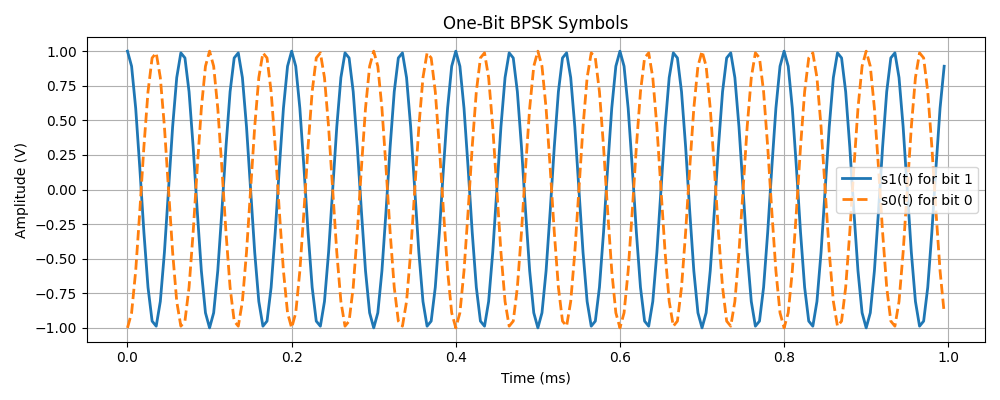
\includegraphics[width=0.8\textwidth]{plots/bpsk.png}
    \caption{BPSK plot}
    \end{figure}